\section{Minimal Automaton}

\textbf{Assumption}: the automaton is clean except for the $q_{err}$ state.

State $p$ is indistinguishable from $q$ iff $\forall x, \delta(p,x)$ and $\delta(q, x)$ are both final or non-final. Indistiguishability is an equivalence relation, 2 indistinguishable states can be merged with no change in the language recognized.

\subsection{Compute distinguishability set}
$p$ is distinguishable from $q$ iff
\begin{itemize}
    \item $p$ is final and $q$ is not, or vice-versa; or
    \item $\exists a: \delta(p, a)$ is distinguishable from $\delta(q, a)$
\end{itemize}

\textbf{Example}
\begin{figure}[H]
    \centering
    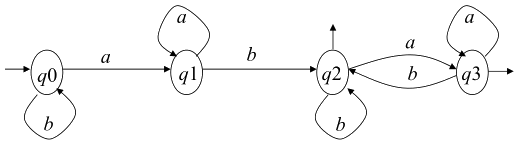
\includegraphics[width=\linewidth]{automata/example-automaton-minimization.png}
\end{figure}

\begin{table}[H]
    \centering
    \begin{minipage}{0.35\linewidth}
        \begin{tabular}{r|c|cc}
            \cline{2-2}
            $q_1$ & & & \\
            \cline{2-3}
            $q_2$ & \xmark & \multicolumn{1}{c|}{\xmark} & \\
            \cline{2-4}
            $q_3$ & \xmark & \multicolumn{1}{c|}{\xmark} & \multicolumn{1}{c|}{} \\
            \cline{2-4}
            \multicolumn{1}{c}{} & \multicolumn{1}{c}{$q_0$} & $q_1$ & $q_2$
        \end{tabular}
    \end{minipage}
    \begin{minipage}{0.6\linewidth}
        \begin{tabular}{r|c|cc}
            \cline{2-2}
            $q_1$ & (1,1)(0,2) & & \\
            \cline{2-3}
            $q_2$ & \xmark & \multicolumn{1}{c|}{\xmark} & \\
            \cline{2-4}
            $q_3$ & \xmark & \multicolumn{1}{c|}{\xmark} & \multicolumn{1}{c|}{(3,3)(2,2)} \\
            \cline{2-4}
            \multicolumn{1}{c}{} & \multicolumn{1}{c}{$q_0$} & $q_1$ & $q_2$
        \end{tabular}
    \end{minipage}
    \begin{minipage}{0.6\linewidth}
        \begin{tabular}{r|c|cc}
            \cline{2-2}
            $q_1$ & \xmark & & \\
            \cline{2-3}
            $q_2$ & \xmark & \multicolumn{1}{c|}{\xmark} & \\
            \cline{2-4}
            $q_3$ & \xmark & \multicolumn{1}{c|}{\xmark} & \multicolumn{1}{c|}{(3,3)(2,2)} \\
            \cline{2-4}
            \multicolumn{1}{c}{} & \multicolumn{1}{c}{$q_0$} & $q_1$ & $q_2$
        \end{tabular}
    \end{minipage}
\end{table}

States $q_2$ and $q_3$ are indistinguishable, so they can be merged.

\begin{figure}[H]
    \centering
    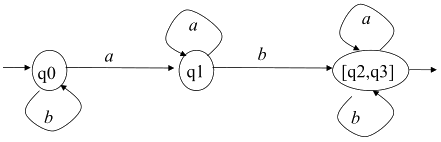
\includegraphics[width=\linewidth]{automata/example-automaton-minimization-2.png}
\end{figure}
